
\subsection{Relative and Incremental Coordinates\\相对和增量坐标}

\subsubsection{Specifying Relative Coordinates\\指定相对坐标}

You can prefix coordinates by |++| to make them ``relative''. A coordinate such
as |++(1cm,0pt)| means ``1cm to the right of the previous position, making this
the new current position''. Relative coordinates are often useful in ``local''
contexts:
 
您可以在坐标前面加上|++|使其成为“相对”坐标。例如,像|++(1cm,0pt)|这样的坐标意味着“相对于前一个位置向右1cm,这成为新的当前位置”。在“局部”环境中,相对坐标通常很有用:

%
\begin{codeexample}[]
\begin{tikzpicture}
  \draw (0,0)     -- ++(1,0) -- ++(0,1) -- ++(-1,0) -- cycle;
  \draw (2,0)     -- ++(1,0) -- ++(0,1) -- ++(-1,0) -- cycle;
  \draw (1.5,1.5) -- ++(1,0) -- ++(0,1) -- ++(-1,0) -- cycle;
\end{tikzpicture}
\end{codeexample}

Instead of |++| you can also use a single |+|. This also specifies a relative
coordinate, but it does not ``update'' the current point for subsequent usages
of relative coordinates. Thus, you can use this notation to specify numerous
points, all relative to the same ``initial'' point:

您也可以使用单个|+|代替|++|。这也指定了一个相对坐标,但它不会“更新”当前点以供后续使用的相对坐标。因此,您可以使用此记法指定多个点,所有这些点都相对于同一个“初始”点:


\begin{codeexample}[]
\begin{tikzpicture}
  \draw (0,0)     -- +(1,0) -- +(1,1) -- +(0,1) -- cycle;
  \draw (2,0)     -- +(1,0) -- +(1,1) -- +(0,1) -- cycle;
  \draw (1.5,1.5) -- +(1,0) -- +(1,1) -- +(0,1) -- cycle;
\end{tikzpicture}
\end{codeexample}

There is a special situation, where relative coordinates are interpreted
differently. If you use a relative coordinate as a control point of a Bézier
curve, the following rule applies: First, a relative first control point is
taken relative to the beginning of the curve. Second, a relative second control
point is taken relative to the end of the curve. Third, a relative end point of
a curve is taken relative to the start of the curve.

有一种特殊情况,其中相对坐标的解释方式不同。如果你将相对坐标用作贝塞尔曲线的控制点,则应遵循以下规则:首先,相对于曲线的起点取相对第一个控制点;其次,相对于曲线的终点取相对第二个控制点;第三,相对于曲线的起点取相对终点。


This special behavior makes it easy to specify that a curve should ``leave or
arrive from a certain direction'' at the start or end. In the following
example, the curve ``leaves'' at $30^\circ$ and ``arrives'' at $60^\circ$:


这种特殊行为使得在起点或终点处指定曲线应该“从某个方向离开或到达”变得容易。在下面的示例中,曲线“离开”时角度为$30^\circ$,而“到达”时角度为$60^\circ$:

%
\begin{codeexample}[]
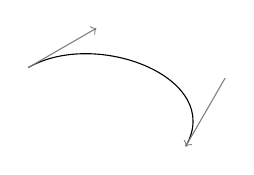
\begin{tikzpicture}
  \draw (1,0) .. controls +(30:1cm) and +(60:1cm) .. (3,-1);
  \draw[gray,->] (1,0) -- +(30:1cm);
  \draw[gray,<-] (3,-1) -- +(60:1cm);
\end{tikzpicture}
\end{codeexample}


\subsubsection{Rotational Relative Coordinates\\旋转相对坐标}

You may sometimes wish to specify points relative not only to the previous
point, but additionally relative to the tangent entering the previous point.
For this, the following key is useful:


有时,你可能希望指定相对于前一个点以及相对于进入前一个点的切线的点。为此,以下关键字很有用:

\begin{key}{/tikz/turn}
    This key can be given as an option to a \meta{coordinate} as in the
    following example:
    
    你可以将该关键字作为选项给出,如下例所示:%
\begin{codeexample}[]
\tikz \draw (0,0) -- (1,1) -- ([turn]-45:1cm) -- ([turn]-30:1cm);
\end{codeexample}
    %
    The effect of this key is to locally shift the coordinate system so that
    the last point reached is at the origin and the coordinate system is
    ``turned'' so that the $x$-axis points in the direction of a tangent
    entering the last point. This means, in effect, that when you use polar
    coordinates of the form \meta{relative angle}|:|\meta{distance} together
    with the |turn| option, you specify a point that lies at \meta{distance}
    from the last point in the direction of the last tangent entering the last
    point, but with a rotation of \meta{relative angle}.

    此关键字的效果是局部移动坐标系,使得到达的最后一个点位于原点,并且坐标系“转动”,使得$x$轴指向进入最后一个点的切线方向。这实际上意味着,当你使用形式为\meta{relative angle}|:|\meta{distance}的极坐标与|turn|选项一起使用时,你指定了一个位于距离最后一个点\meta{distance}、方向为进入最后一个点的切线方向、旋转角为\meta{relative angle}的点。


    This key also works with curves \dots

    该关键字还适用于曲线……

    %
\begin{codeexample}[]
\tikz [delta angle=30, radius=1cm]
  \draw (0,0) arc [start angle=0]  -- ([turn]0:1cm)
              arc [start angle=30] -- ([turn]0:1cm)
              arc [start angle=60] -- ([turn]30:1cm);
\end{codeexample}
\begin{codeexample}[]
\tikz \draw (0,0) to [bend left] (2,1) -- ([turn]0:1cm);
\end{codeexample}
    %
    \dots and with plots \dots

    ……以及绘图……
    %
\begin{codeexample}[]
\tikz \draw plot coordinates {(0,0) (1,1) (2,0) (3,0) } -- ([turn]30:1cm);
\end{codeexample}

    Although the above examples use polar coordinates with |turn|, you can also
    use any normal coordinate. For instance, |([turn]1,1)| will append a line
    of length $\sqrt 2$ that is turns by $45^\circ$ relative to the tangent to
    the last point.
    %

    虽然上面的示例使用了带有|turn|的极坐标,但你也可以使用任何普通坐标。例如,|([turn]1,1)| 将附加一条长度为 $\sqrt 2$ 的线,相对于最后一个点的切线旋转 $45^\circ$。
\begin{codeexample}[]
\tikz \draw (0.5,0.5) -| (2,1) -- ([turn]1,1)
         .. controls ([turn]0:1cm) .. ([turn]-90:1cm);
\end{codeexample}
    %
\end{key}


\subsubsection{Relative Coordinates and Scopes\\相对坐标和作用域}
\label{section-scopes-relative}

An interesting question is, how do relative coordinates behave in the presence
of scopes? That is, suppose we use curly braces in a path to make part of it
``local'', how does that affect the current position? On the one hand, the
current position certainly changes since the scope only affects options, not
the path itself. On the other hand, it may be useful to ``temporarily escape''
from the updating of the current point.

一个有趣的问题是,在作用域存在的情况下,相对坐标的行为如何?也就是说,假设我们在路径中使用花括号使其的一部分“局部化”,那么这将如何影响当前位置呢?一方面,当前位置肯定会发生变化,因为作用域只影响选项,而不影响路径本身。另一方面,暂时“逃离”当前点的更新可能是有用的。


Since both interpretations of how the current point and scopes should
``interact'' are useful, there is a (local!) option that allows you to decide
which you need.

由于当前点和作用域应如何“交互”的这两种解释都是有用的,因此有一个(局部的!)选项可以让你决定你需要哪种方式。


\begin{key}{/tikz/current point is local=\opt{\meta{boolean}} (initially false)}
    Normally, the scope path operation has no effect on the current point. That
    is, curly braces on a path have no effect on the current position:
    
    通常来说,作用域路径操作对当前点没有影响。也就是说,路径中的花括号对当前位置没有影响:
%
\begin{codeexample}[]
\begin{tikzpicture}
  \draw      (0,0) -- ++(1,0)   -- ++(0,1)   -- ++(-1,0);
  \draw[red] (2,0) -- ++(1,0) { -- ++(0,1) } -- ++(-1,0);
\end{tikzpicture}
\end{codeexample}
    %
    If you set this key to |true|, this behavior changes. In this case, at the
    end of a group created on a path, the last current position reverts to
    whatever value it had at the beginning of the scope. More precisely, when
    \tikzname\ encounters |}| on a path, it checks whether at this particular
    moment the key is set to |true|. If so, the current position reverts to the
    value it had when the matching |{| was read.
    
    如果将此关键字设置为 |true|,则此行为会发生变化。在这种情况下,在路径上的一个组的末尾,当前位置将恢复为与读取相匹配的 |{| 时的值。更准确地说,当 \tikzname\ 在路径上遇到 |}| 时,它会检查此时该关键字是否设置为 |true|。如果是,则当前位置将恢复为读取匹配的 |{| 时的值。

%
\begin{codeexample}[]
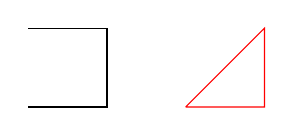
\begin{tikzpicture}
  \draw      (0,0) -- ++(1,0)   -- ++(0,1)   -- ++(-1,0);
  \draw[red] (2,0) -- ++(1,0)
     { [current point is local] -- ++(0,1) } -- ++(-1,0);
\end{tikzpicture}
\end{codeexample}
    %
    In the above example, we could also have given the option outside the
    scope, for instance as a parameter to the whole scope.

    在上面的示例中,我们也可以在作用域之外给出选项,例如作为整个作用域的参数。
\end{key}


\subsection{Coordinate Calculations\\坐标计算}
\label{tikz-lib-calc}

\begin{tikzlibrary}{calc}
    You need to load this library in order to use the coordinate calculation
    functions described in the present section.

    在使用本节中描述的坐标计算函数之前,您需要加载此库。
\end{tikzlibrary}

It is possible to do some basic calculations that involve coordinates. In
essence, you can add and subtract coordinates, scale them, compute midpoints,
and do projections. For instance, |($(a) + 1/3*(1cm,0)$)| is the coordinate
that is $1/3 \text{cm}$ to the right of the point |a|:


可以进行涉及坐标的基本计算。基本上,可以添加和减去坐标,对其进行缩放,计算中点和投影。例如,|($(a) + 1/3*(1cm,0)$)| 是点 |a| 右侧 $1/3 \text{cm}$ 处的坐标:
%
\begin{codeexample}[preamble={\usetikzlibrary{calc}}]
\begin{tikzpicture}
  \draw [help lines] (0,0) grid (3,2);

  \node (a) at (1,1) {A};
  \fill [red] ($(a) + 1/3*(1cm,0)$) circle (2pt);
\end{tikzpicture}
\end{codeexample}


\subsubsection{The General Syntax\\通用语法}

The general syntax is the following:

通用语法如下:
%
\begin{quote}
    \declare{|(|\opt{|[|\meta{options}|]|}|$|\meta{coordinate computation}|$)|}.
\end{quote}

As you can see, the syntax uses the \TeX\ math symbol |$| to %$
indicate that a ``mathematical computation'' is involved. However, the |$| %$
has no other effect, in particular, no mathematical text is typeset.

如您所见,语法使用 \TeX\ 数学符号 |$| 表示涉及``数学计算''。但是,|$| 没有其他作用,特别是没有进行数学文本排版。


The \meta{coordinate computation} has the following structure:

\meta{坐标计算} 具有以下结构:
%
\begin{enumerate}
    \item It starts with
        %

        以如下形式开始:
        \begin{quote}
            \opt{\meta{factor}|*|}\meta{coordinate}\opt{\meta{modifiers}}
        \end{quote}
    \item This is optionally followed by |+| or |-| and then another

    可选地后跟 |+| 或 |-|,然后是另一个
        %
        \begin{quote}
            \opt{\meta{factor}|*|}\meta{coordinate}\opt{\meta{modifiers}}
        \end{quote}
    \item This is once more followed by |+| or |-| and another of the above
        modified coordinate; and so on.

        再次后跟 |+| 或 |-| 和上述修饰过的坐标;以此类推。
\end{enumerate}

In the following, the syntax of factors and of the different modifiers
is explained in detail.

接下来,详细解释因子和不同修饰符的语法。


\subsubsection{The Syntax of Factors\\因子的语法}

The \meta{factor}s are optional and detected by checking whether the
\meta{coordinate computation} starts with a |(|. Also, after each $\pm$ a
\meta{factor} is present if, and only if, the |+| or |-| sign is not directly
followed by~|(|.

\meta{因子}是可选的,通过检查 \meta{坐标计算} 是否以 |(| 开头来确定。此外,在每个 $\pm$ 后,只有在 |+| 或 |-| 符号直接后面没有跟随 |(| 时才出现 \meta{因子}。

If a \meta{factor} is present, it is evaluated using the |\pgfmathparse| macro.
This means that you can use pretty complicated computations inside a factor. A
\meta{factor} may even contain opening parentheses, which creates a
complication: How does \tikzname\ know where a \meta{factor} ends and where a
coordinate starts? For instance, if the beginning of a \meta{coordinate
computation} is |2*(3+4|\dots, it is not clear whether |3+4| is part of a
\meta{coordinate} or part of a \meta{factor}. Because of this, the following
rule is used: Once it has been determined, that a \meta{factor} is present, in
principle, the \meta{factor} contains everything up to the next occurrence of
|*(|. Note that there is no space between the asterisk and the parenthesis.

如果存在 \meta{因子},则使用 |\pgfmathparse| 宏对其进行求值。这意味着您可以在因子内使用相当复杂的计算。一个 \meta{因子} 甚至可以包含括号,这会导致一个问题:\tikzname\ 如何知道 \meta{因子} 在哪里结束,坐标从哪里开始?例如,如果 \meta{坐标计算} 的开头是 |2*(3+4|\dots,不清楚 |3+4| 是 \meta{坐标} 的一部分还是 \meta{因子} 的一部分。因此,采用以下规则:一旦确定存在 \meta{因子},原则上,\meta{因子} 包含直到下一个出现的 |*(| 为止。请注意,星号和括号之间没有空格。

It is permissible to put the \meta{factor} in curly braces. This can be used
whenever it is unclear where the \meta{factor} would end.

可以将 \meta{因子} 放在花括号中。这可以在不清楚 \meta{因子} 结束的地方使用。

Here are some examples of coordinate specifications that consist of exactly one
\meta{factor} and one \meta{coordinate}:

以下是由一个 \meta{因子} 和一个 \meta{坐标} 组成的坐标规范的示例:

%
\begin{codeexample}[preamble={\usetikzlibrary{calc}}]
\begin{tikzpicture}
  \draw [help lines] (0,0) grid (3,2);

  \fill [red] ($2*(1,1)$) circle (2pt);
  \fill [green] (${1+1}*(1,.5)$) circle (2pt);
  \fill [blue] ($cos(0)*sin(90)*(1,1)$) circle (2pt);
  \fill [black] (${3*(4-3)}*(1,0.5)$) circle (2pt);
\end{tikzpicture}
\end{codeexample}


\subsubsection{The Syntax of Partway Modifiers\\部分修饰符的语法}

A \meta{coordinate} can be followed by different \meta{modifiers}. The first
kind of modifier is the \emph{partway modifier}. The syntax (which is loosely
inspired by Uwe Kern's |xcolor| package) is the following:

\meta{坐标}可以后跟不同的\meta{修饰符}。第一种修饰符是\emph{部分修饰符}。其语法(受Uwe Kern的|xcolor|宏包的启发,但略有不同)如下:
%
\begin{quote}
    \meta{coordinate}\declare{|!|\meta{number}|!|\opt{\meta{angle}|:|}\meta{second coordinate}}
\end{quote}
%
One could write for instance

例如,可以写作:
%
\begin{codeexample}[code only]
(1,2)!.75!(3,4)
\end{codeexample}
%
The meaning of this is: ``Use the coordinate that is three quarters on the way
from |(1,2)| to |(3,4)|.'' In general, \meta{coordinate
x}|!|\meta{number}|!|\meta{coordinate y} yields the coordinate $(1 -
\meta{number})\meta{coordinate x} + \meta{number} \meta{coordinate y}$. Note
that this is a bit different from the way the \meta{number} is interpreted in
the |xcolor| package: First, you use a factor between $0$ and $1$, not a
percentage, and, second, as the \meta{number} approaches $1$, we approach the
second coordinate, not the first. It is permissible to use a \meta{number} that
is smaller than $0$ or larger than $1$. The \meta{number} is evaluated using
the |\pgfmathparse| command and, thus, it can involve complicated computations.


它的含义是:“使用从|(1,2)|到|(3,4)|的路径的四分之三的位置上的坐标。” 一般而言,\meta{坐标x}|!|\meta{数值}|!|\meta{坐标y}将生成坐标$(1-\meta{数值})\meta{坐标x} + \meta{数值}\meta{坐标y}$。需要注意的是,这与|xcolor|宏包中对\meta{数值}的解释有所不同:首先,使用的是0到1之间的因子,而不是百分比;其次,当\meta{数值}趋近于1时,接近第二个坐标,而不是第一个坐标。可以使用小于0或大于1的\meta{数值}。\meta{数值}通过|\pgfmathparse|命令计算,因此可以涉及复杂的计算。
%
\begin{codeexample}[preamble={\usetikzlibrary{calc}}]
\begin{tikzpicture}
  \draw [help lines] (0,0) grid (3,2);

  \draw (1,0) -- (3,2);

  \foreach \i in {0,0.2,0.5,0.9,1}
    \node at ($(1,0)!\i!(3,2)$) {\i};
\end{tikzpicture}
\end{codeexample}

The \meta{second coordinate} may be prefixed by an \meta{angle}, separated with
a colon, as in |(1,1)!.5!60:(2,2)|. The general meaning of
\meta{a}|!|\meta{factor}|!|\meta{angle}|:|\meta{b} is: ``First, consider the
line from \meta{a} to \meta{b}. Then rotate this line by \meta{angle}
\emph{around the point \meta{a}}. Then the two endpoints of this line will be
\meta{a} and some point \meta{c}. Use this point \meta{c} for the subsequent
computation, namely the partway computation.''

\meta{第二个坐标}可以带有前缀\meta{角度},用冒号分隔,例如 |(1,1)!.5!60:(2,2)|。\meta{a}|!|\meta{因子}|!|\meta{角度}|:|\meta{b}的一般含义是:“首先,考虑从\meta{a}到\meta{b}的直线。然后以\meta{a}为中心,将这条直线旋转\meta{角度}。这条直线的两个端点将是\meta{a}和某个点\meta{c}。使用该点\meta{c}进行后续计算,即部分计算。”

Here are two examples:

以下是两个示例:
%
\begin{codeexample}[preamble={\usetikzlibrary{calc}}]
\begin{tikzpicture}
  \draw [help lines] (0,0) grid (3,3);

  \coordinate (a) at (1,0);
  \coordinate (b) at (3,2);

  \draw[->] (a) -- (b);

  \coordinate (c) at ($ (a)!1! 10:(b) $);

  \draw[->,red] (a) -- (c);

  \fill ($ (a)!.5! 10:(b) $) circle (2pt);
\end{tikzpicture}
\end{codeexample}

\begin{codeexample}[preamble={\usetikzlibrary{calc}}]
\begin{tikzpicture}
  \draw [help lines] (0,0) grid (4,4);

  \foreach \i in {0,0.1,...,2}
    \fill ($(2,2) !\i! \i*180:(3,2)$) circle (2pt);
\end{tikzpicture}
\end{codeexample}

You can repeatedly apply modifiers. That is, after any modifier you can add
another (possibly different) modifier.

可以重复应用修饰符。也就是说,在任何修饰符之后,可以添加另一个(可能不同的)修饰符。
%
\begin{codeexample}[preamble={\usetikzlibrary{calc}}]
\begin{tikzpicture}
  \draw [help lines] (0,0) grid (3,2);

  \draw (0,0) -- (3,2);
  \draw[red] ($(0,0)!.3!(3,2)$) -- (3,0);
  \fill[red] ($(0,0)!.3!(3,2)!.7!(3,0)$) circle (2pt);
\end{tikzpicture}
\end{codeexample}


\subsubsection{The Syntax of Distance Modifiers\\部分修饰符的语法}

A \emph{distance modifier} has nearly the same syntax as a partway modifier,
only you use a \meta{dimension} (something like |1cm|) instead of a
\meta{factor} (something like |0.5|):

一个\emph{距离修饰符}的语法几乎与\emph{部分修饰符}相同,只是你使用一个\meta{dimension}(类似于|1cm|的东西)而不是\meta{factor}(类似于|0.5|):


%
\begin{quote}
    \meta{coordinate}\declare{|!|\meta{dimension}|!|\opt{\meta{angle}|:|}\meta{second coordinate}}
\end{quote}

When you write \meta{a}|!|\meta{dimension}|!|\meta{b}, this means the
following: Use the point that is distanced \meta{dimension} from \meta{a} on
the straight line from \meta{a} to \meta{b}. Here is an example:

当你写下\meta{a}|!|\meta{dimension}|!|\meta{b}时,意味着以下内容:在从\meta{a}到\meta{b}的直线上,距离\meta{a} \meta{dimension}的点。以下是一个示例:

%
\begin{codeexample}[preamble={\usetikzlibrary{calc}}]
\begin{tikzpicture}
  \draw [help lines] (0,0) grid (3,2);

  \draw (1,0) -- (3,2);

  \foreach \i in {0cm,1cm,15mm}
    \node at ($(1,0)!\i!(3,2)$) {\i};
\end{tikzpicture}
\end{codeexample}

As before, if you use a \meta{angle}, the \meta{second coordinate} is rotated
by this much around the \meta{coordinate} before it is used.

与之前一样,如果使用\meta{angle},\meta{second coordinate}在使用之前会旋转这么多。

The combination of an \meta{angle} of |90| degrees with a distance can be used
to ``offset'' a point relative to a line. Suppose, for instance, that you have
computed a point |(c)| that lies somewhere on a line from |(a)| to~|(b)| and
you now wish to offset this point by |1cm| so that the distance from this
offset point to the line is |1cm|. This can be achieved as follows:

将\meta{angle}为|90|度与一个距离结合起来,可以用于相对于一条直线进行“偏移”一个点。例如,假设你计算出一个点|(c)|位于从|(a)|到|(b)|的某条线上,现在你希望将此点偏移|1cm|,使得该偏移点到该线的距离为|1cm|。可以按如下方式实现:

%
\begin{codeexample}[preamble={\usetikzlibrary{calc}}]
\begin{tikzpicture}
  \draw [help lines] (0,0) grid (3,2);

  \coordinate (a) at (1,0);
  \coordinate (b) at (3,1);

  \draw (a) -- (b);

  \coordinate (c) at ($ (a)!.25!(b) $);
  \coordinate (d) at ($ (c)!1cm!90:(b) $);

  \draw [<->] (c) -- (d) node [sloped,midway,above] {1cm};
\end{tikzpicture}
\end{codeexample}


\subsubsection{The Syntax of Projection Modifiers\\投影修饰符的语法}

The projection modifier is also similar to the above modifiers: It also gives a
point on a line from the \meta{coordinate} to the \meta{second coordinate}.
However, the \meta{number} or \meta{dimension} is replaced by a
\meta{projection coordinate}:


投影修饰符与上述修饰符类似:它也会给出从\meta{坐标}到\meta{第二个坐标}的线上的一个点。然而,\meta{数字}或\meta{尺寸}被替换为\meta{投影坐标}:
%
\begin{quote}
    \meta{coordinate}\declare{|!|\meta{projection coordinate}|!|\opt{\meta{angle}|:|}\meta{second coordinate}}
\end{quote}

Here is an example:

下面是一个示例:
%
\begin{codeexample}[code only]
(1,2)!(0,5)!(3,4)
\end{codeexample}

The effect is the following: We project the \meta{projection coordinate}
orthogonally onto the line from \meta{coordinate} to \meta{second coordinate}.
This makes it easy to compute projected points:

效果如下:我们将\meta{投影坐标}在垂直于从\meta{坐标}到\meta{第二个坐标}的直线上进行投影。这使得计算投影点变得容易:
%
\begin{codeexample}[preamble={\usetikzlibrary{calc}}]
\begin{tikzpicture}
  \draw [help lines] (0,0) grid (3,2);

  \coordinate (a) at (0,1);
  \coordinate (b) at (3,2);
  \coordinate (c) at (2.5,0);

  \draw (a) -- (b) -- (c) -- cycle;

  \draw[red]    (a) -- ($(b)!(a)!(c)$);
  \draw[orange] (b) -- ($(a)!(b)!(c)$);
  \draw[blue]   (c) -- ($(a)!(c)!(b)$);
\end{tikzpicture}
\end{codeexample}
